\documentclass[conference]{IEEEtran}
% zvolte kodovani
\usepackage[utf8]{inputenc}
\usepackage{fullpage}
\usepackage{graphicx}
\usepackage{amsmath}
\usepackage{float}
\usepackage{epstopdf}
\usepackage{todonotes}
\usepackage{hyperref}
\usepackage{parskip}
\usepackage[justification=centering]{caption}
\setlength{\belowcaptionskip}{-7pt}

\begin{document}

\title{Genetic Clustering for the Multi-depot Vehicle Routing Problem}
\author{Libor Novák}

\maketitle

\begin{abstract}
In this project, the multi depot vehicle routing problem (MDVRP) is examined. The task is split into two subsidiary tasks. First, the customers are clustered in order to determine the depot from which each customer will be served. Then, the classical vehicle routing problem (VRP) is applied and solved for each of the clusters. The goal of this project is to suggest a new clustering method based on genetic algorithms for solving the first part of the MDVRP task.
\end{abstract}

\IEEEpeerreviewmaketitle


\section{Assignment}
One way to approach the Multi Depot Vehicle Routing Problem (MDVRP) is to employ two steps. First, the customers are clustered - assigned to each depot and, subsequently, for each cluster the classical Vehicle Routing Problem (VRP) is solved. Because the cluster centers are in this case given by the positions of the depots, all regular clustering methods yield the same solutions, which does not have to be ideal for the final solution of this task. Suggest, implement and test a new clustering method specifically for the MDVRP using genetic algorithms.



\section{Introduction}
The vehicle routing problem (VRP) is a task, where, given a set of customers $C$ and a depot, we are asked to determine the optimal routes of trucks to serve these customers and return to the depot. The goal is to minimize the cost of travel in terms of distance traveled, while meeting other constraints. The multi depot vehicle routing problem (MDVRP) is an extension of the basic problem, where we consider the customers to be served from several available depots $d_m \in D$. The positions of the customers $c_n \in C$ and the positions of the depots $d_m \in D$ are specified as well as the routes and the lengths $r_{ij}; i,j \in C \cup D$ between the customers and the depots.

In this semestral work we will address the problem of clustering the customers. The VRP for each depot is simplified to the Traveling Salesman Problem (TSP) since we do not consider maximum capacity of each truck. Therefore one truck is considered for each depot. The only constraint we consider is the maximum supply of each depot, excluding this constraint would lead to always having one single cluster of all customers. 

The importance of the used clustering method is obvious. Once we create the clusters, the VRP can only solve the subtasks within those clusters, therefore optimal clustering of the customers is crucial to obtain good results of the MDVRP. In most cases, the customers are assigned to the closest depot (given Euclidean distance) available as in Surekha and Sumathi \cite{surekha2011solution}, which is nothing more than K-Means clustering. This is possible because the distances between the customers $c_n$ and the depots $d_m$ are given by their Euclidean distance on a 2D map
$$
\text{dst}(c_i, d_j) = \| p(c_i) - p(d_j) \|,
$$
where $p(.)$ denotes the position on the map and the map can be represented as a complete undirected graph. Nevertheless, in this clustering approach the total demand of the customers in each cluster (the workload of each depot) is not considered, neither are the distances between the customers themselves. 

In this semestral project, we exploit the adaptability of genetic algorithms and suggest a new clustering method for the MDVRP. In the next section, the optimization problem is stated and the genetic algorithm described, followed by comparison of obtained results in the subsequent section, followed by discussion.



\section{Problem Statement and Solution}

\subsection{Problem Statement}
We are solving a special case of the MDVRP, where we consider only one truck to be launched from each depot. Therefore for the set of trucks $T$ it holds that $|T| = |D|$, i.e. the number of trucks is the same as the number of depots. The goal is to minimize the total route length, which can be stated as
\begin{align*}
  &\min \sum_{i=1}^{|T|} r_{i}, \\
  &\text{s.t. } dem(d_i) \leq Thr \qquad \forall i = 1,...,|D|,
\end{align*}
where $r_{i}$ is the length of the route of the truck $i$ and $dem(d_i)$ is the demand covered by the depot $d_i$, which has to be lower or equal to the maximum depot coverage $Thr$.

The MDVRP is a NP hard problem, therefore several heuristics are used in order to make this task solvable in a reasonable time frame. The usual heuristic used to approach MDVRP is to split the customers $C = C_1 \cup C_2 \cup ... \cup C_{|D|}$ into several sets - clusters $d_m \in D$, which are assigned to depots (each set of customers $C_m \subset C$ is served by exactly one depot $d_m$). This simplifies the problem to $|D|$ VRPs, which are then solvable either using direct tree search methods, linear programming, Clarke and Wright \cite{clarke1964scheduling} method or other, as described by Laporte \cite{laporte1992vehicle}. In this semestral work we use the Clarke and Wright method.

The clustering itself is of a special kind because we are not seeking the optimal positions of the cluster centers as in the classical clustering task, but the cluster centers are given by the depot positions $p(d_m)$. We seek the optimal assignment of the customers $c_n \in C$ to the depots $d_m \in D$. This difference is however crucial, the most commonly used K-means, EM and graph clustering methods \cite{alldrin2003clustering} assign the customers always to the closest center, therefore yielding the same results. These approaches can be disadvantageous when the depots are not evenly distributed over the map.


\subsection{Solution} % (fold)
\label{sub:solution}
Since we would like to examine the possibility of creating different kinds of clusters, we will make use of the flexibility of genetic algorithms, i.e. their fitness functions, which allows us to specify different clustering objectives than just distance to the depot (cluster center). Several versions and ideas can be found in \cite{pelikan2000genetic,murthy1996search}.

For our experiments, we used an altered version of the general genetic algorithm, as described in Figure \ref{gapscd}.
\begin{figure}[b]
    \hrulefill\\
  Randomly initialize population. \\
  Repair the individuals in the population.\\
  For $g = 1,...,G$: 
  \begin{itemize}
    \item Compute fitness of all individuals.
    \item Elitism.
    \item Tournament selection.
    \item Uniform crossover.
    \item Mutation.
    \item Repair the individuals.
    \item Replace the whole population.
  \end{itemize}
  Output the best individual.

  \hrulefill
    \caption{Genetic algorithm for clustering, pseudo code.}
    \label{gapscd}
\end{figure}

\paragraph{Representation} Each individual in the population is an assignment of the customers to the depots, that is its chromosome is for example $[1,4,2,3,3,2,4]$, where the position (locus) is the customer index and the number at that position (gene) is the depot index to which the customer is assigned.

\paragraph{Initialization} The population is initialized randomly with equiprobable distribution.

\paragraph{Elitism} From each population, we directly select the individual with the best fitness for mating.

\paragraph{Selection} Tournament selection is used in our implementation, where the best out of 5 randomly selected individuals is chosen as a future parent.

\paragraph{Crossover} Each pair of parents has a probability of undergoing crossover. We use uniform crossover - for each locus we determine with probability 0.5 whether the gene of the individuals will be kept or swapped. Both children are then added to the new population.

\paragraph{Mutation} After a new population is generated by selection and crossover, the individuals go through mutation with certain probability. We use a simple bit flip, which means that each locus has a certain probability to experience mutation and if mutation is carried out for the given locus, then we randomly select one depot (gene) to be put in that position.

\paragraph{Replacement} The whole population is then replaced with the newly generated individuals - generational replacement.


One can notice that there is an extra step in the pseudo code (Figure \ref{gapscd}) for repairing the population. This step assures that all individuals in the population meet the condition on the maximum capacity of the depots. We created a function that carries out the fixing, which is described in Figure \ref{reppscd}.
\begin{figure}[b]
    \hrulefill\\
  Given: $D = \{d_1,...,d_m\}$, $C_i = \{c_{i1},...,c_{in_i}\}, max\_demand$ \\
  Initialize $D_e = \{\text{all depots exceeding their capacity}\}$. \\
  While $not empty(D_e)$: 
  \begin{itemize}
    \item Take a depot $i$ from $D_e$.
    \item Random shuffle customers $C_i$.
    \item While $demand(d_i) > max\_demand$
    \begin{itemize}
      \item For $j = 1,...,n_i$: 
      \begin{itemize}
        \item Try to place the customer $c_{ij}$ into one of the depots from $D \setminus D_e$.
        \item If it is possible, move it, otherwise leave it in the depot $d_i$.
      \end{itemize}
    \end{itemize}
    \item Remove $d_i$ from $D_e$. $D_e = D_e \setminus \{d_i\}$.
  \end{itemize}

  \hrulefill
    \caption{Individual fixing process.}
    \label{reppscd}
\end{figure}
% subsection solution (end)

\subsection{Fitness Computation - Exclusive Pairing} % (fold)
\label{sub:fitness_computation_exclusive_pairing}
We propose a new fitness function that uses nearly exclusive pairing of the customers assigned to each depot. The motivation behind it is to assimilate the routing process without actually solving it. Instead of taking into account the distance of the customers to the cluster center, we use the distance between the customers themselves.

We pair the customers in each cluster according to their distance (closest ones are a pair), however once we pair a customer with another one, the latter cannot select the former as its pair anymore, therefore perhaps the second nearest must be selected as the paired one.

Let us have one individual, denote $C_i$ the set of customers assigned to the depot $d_i$. For simplicity we will describe only individual in one generation and therefore leave out the subscripts of the generation and indices denoting the individual. Denote $CM_i$ the set of already paired customers served by the depot $d_i$, which is empty in the beginning. For each depot we randomly order the customers. Then we take one by one customer $c_{ij}$ and always select the closest neighbor (customer) from the set of not yet paired customers $C_i \setminus CM_i$. Add their distance to the total fitness function and add the customer $c_{ij}$ to $CM_i$. This is done for all customers and all depots. Pseudo code is shown in Figure \ref{pseudocode}.
\begin{figure}
    \hrulefill\\
  Given: $D = \{d_1,...,d_m\}$, $C_i = \{c_{i1},...,c_{in_i}\}$ \\
  Initialize $fitness = 0$. \\
  For $i = 1,...,m$: 
  \begin{itemize}
    \item Random shuffle customers $C_i$.
    \item Set $CM_i = \emptyset$.
    \item For $j = 1,...,n_i$: 
    \begin{itemize}
      \item Find the closest customer $c_{ic}$ to the customer $c_{ij}$ from the set $C_i \setminus CM_i$.
      \item Add the distance $d(c_{ic},c_{ij})$ to the total fitness function
      \[
        fitness = fitness + d(c_{ic},c_{ij}).
      \]
      \item Set the current customer as already paired $CM_i = CM_i \cup \{c_{ij}\}$.
    \end{itemize}
  \end{itemize}
  Output $fitness$.

  \hrulefill
    \caption{Exclusive Pairing fitness computation pseudo code.}
    \label{pseudocode}
\end{figure}

We then minimize this fitness function. It can be noticed that the exclusivity of the pairing in the fitness function is questionable because there can be more customers, which have the same nearest neighbor. Here we exclude only mutually nearest neighbors, which as an approximation works well.

Because the value of the fitness function actually depends on the order in which the customers are paired, we carry out this computation several times with different random orderings of the customers, which gives us a higher chance of finding a value, which is closer to the optimum. This method can be understood as a variant of RANSAC \cite{fischler1981random}.
% subsection fitness_computation_exclusive_pairing (end)



\section{Experiments}
For testing we used the set of Cordeau's instances (\url{http://www.bernabe.dorronsoro.es/vrp/}), which is a well known benchmark for MDVRP that was also used for instance by Surekha and Sumanthi \cite{surekha2011solution}. It contains several problems from several up to hundredths of customers. We present our results on the instances \texttt{p07} (Figure \ref{p07datas}) and \texttt{p07altered} (Figure \ref{p03datas}), where we modified the positions of the depots.
\begin{figure*}
  \centering
  \begin{minipage}[t]{0.49\textwidth}
    \begin{center}
      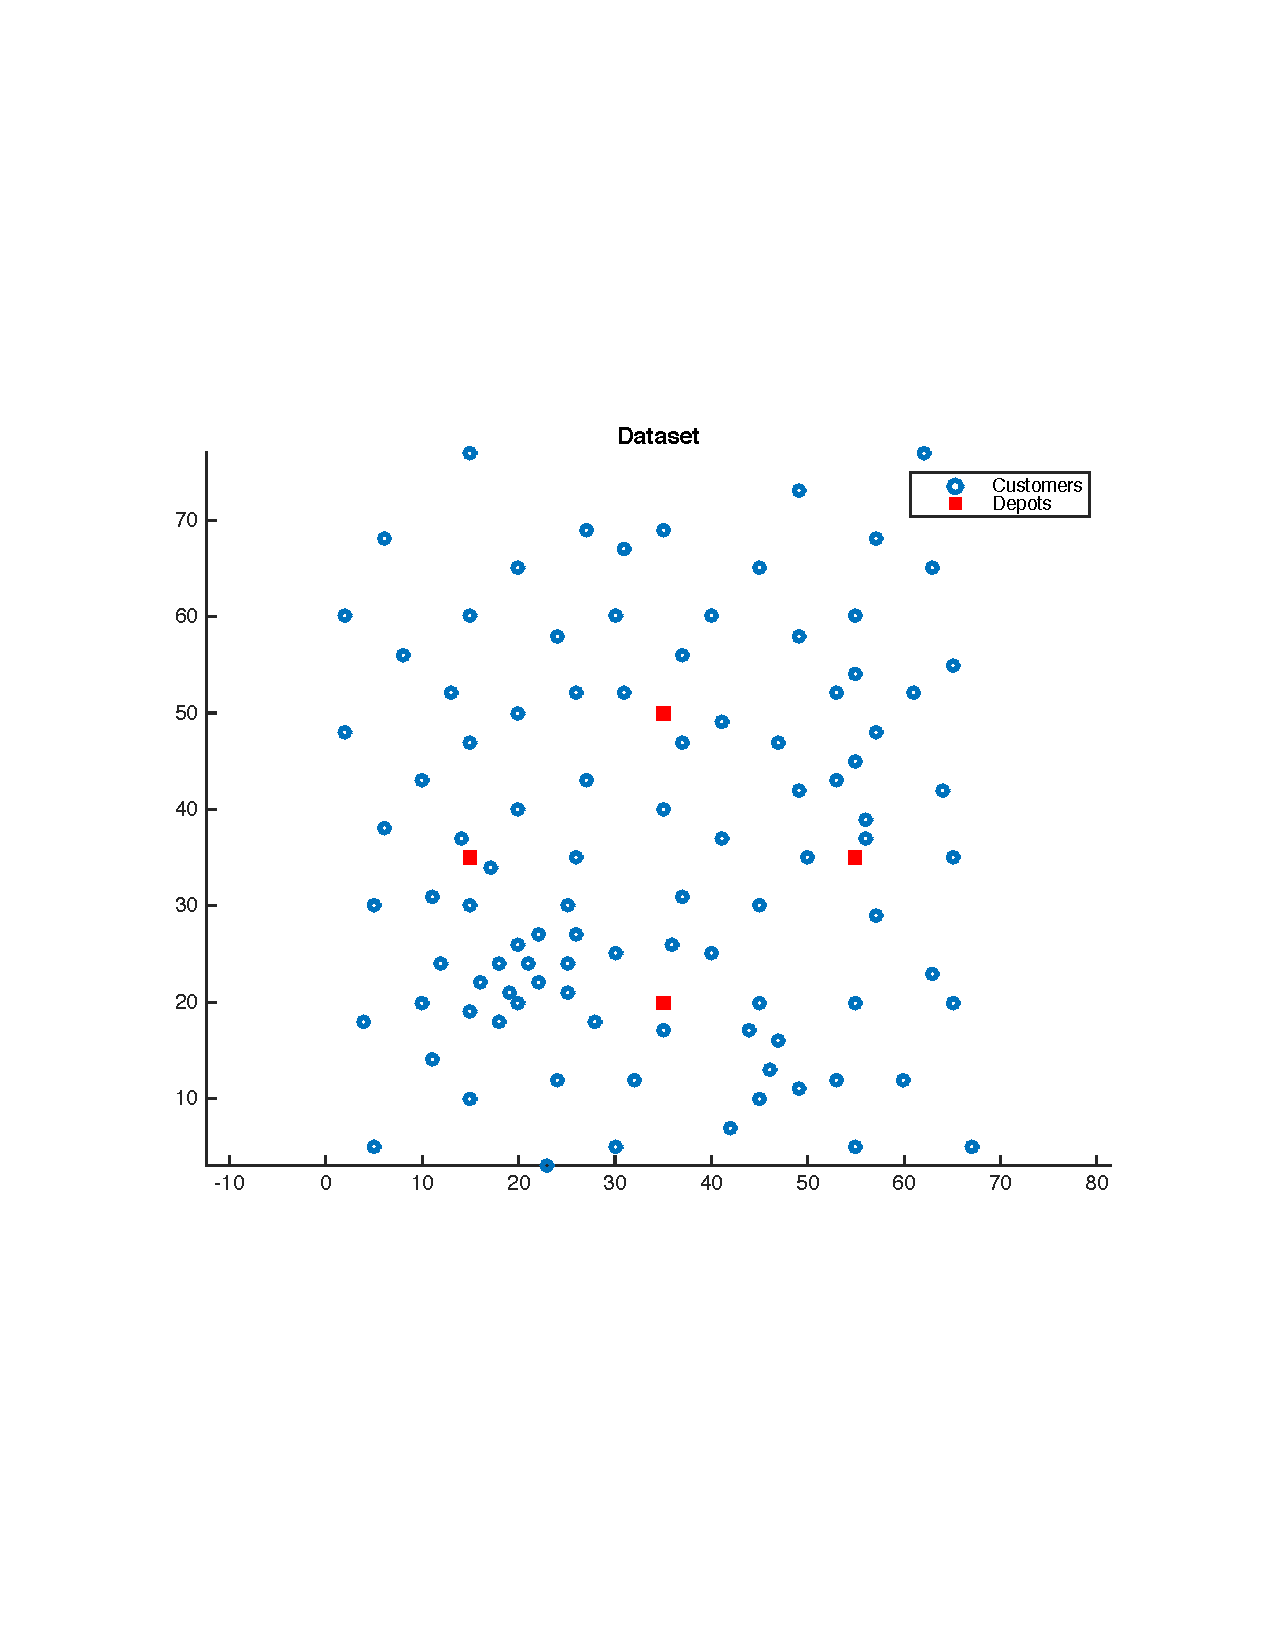
\includegraphics[width=4cm]{images/p07dataset}
      \caption{Cordeau's instance \texttt{p07}}
      \label{p07datas}
    \end{center}
  \end{minipage}
  \hfill
  \begin{minipage}[t]{0.49\textwidth}
    \begin{center}
      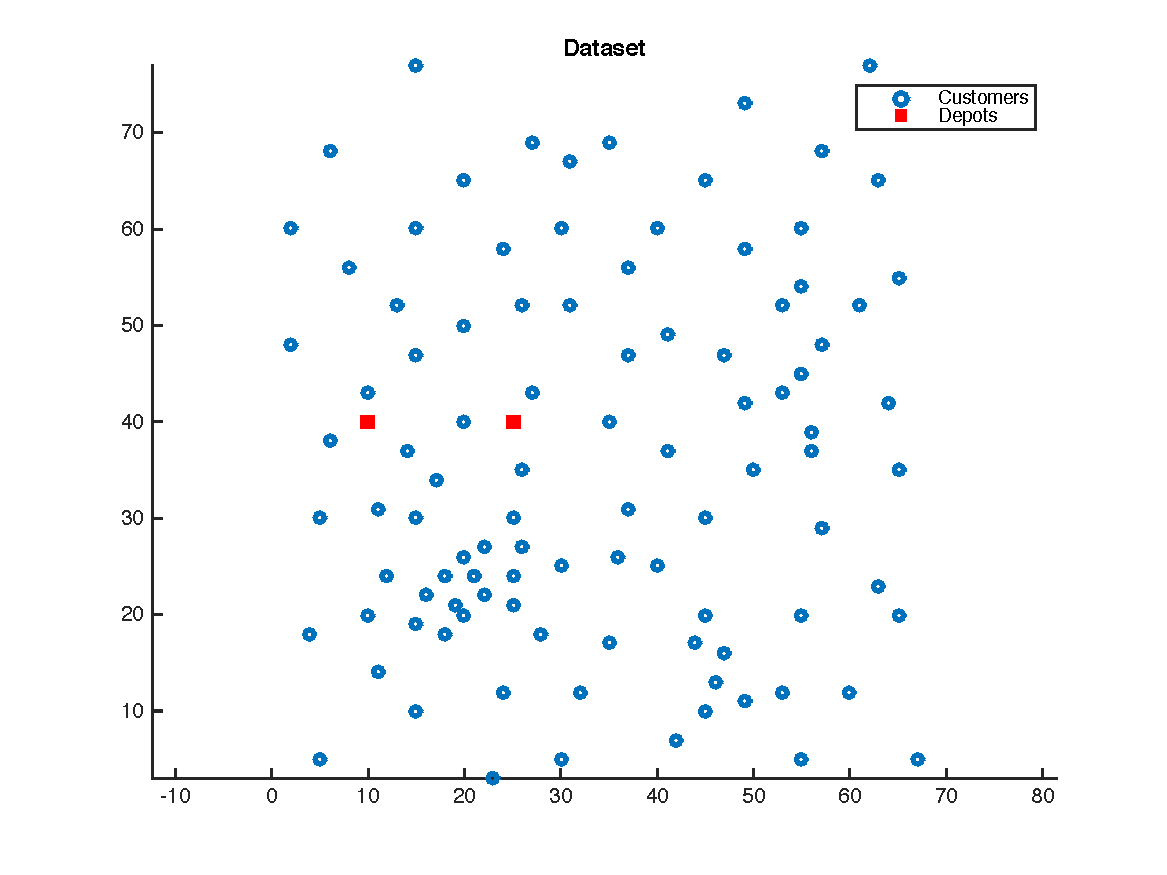
\includegraphics[width=4cm]{images/p07altereddataset}
      \caption{Cordeau's instance \texttt{p07altered}}
      \label{p03datas}
    \end{center}
  \end{minipage}
\end{figure*}

We performed three runs through clustering since the results differ for each run due to randomness of genetic algorithms. We then took the best found solution and compared with each other. In each run we used the population of 100 individuals and the evolution was ran for 99 generations. The probability of crossover was set to 0.8 and the probability of mutation of each gene to 0.02. The tournament selection was carried out on 5 randomly selected individuals.

As a baseline we took K-Means clustering. In fact, the regular K-Means clustering could not be used since it does not take into account the maximum depot capacity constraint. Therefore a genetic algorithm with a fitness function - Distance to The Depot was used to assimilate K-Means clustering. The results of this method are shown in Figure \ref{n1res}. On the left, we can see the clusters created by this method, middle shows the solution to the MDVRP. On the right we see how the fitness evolved in each population.
\begin{figure*}
  \begin{center}
    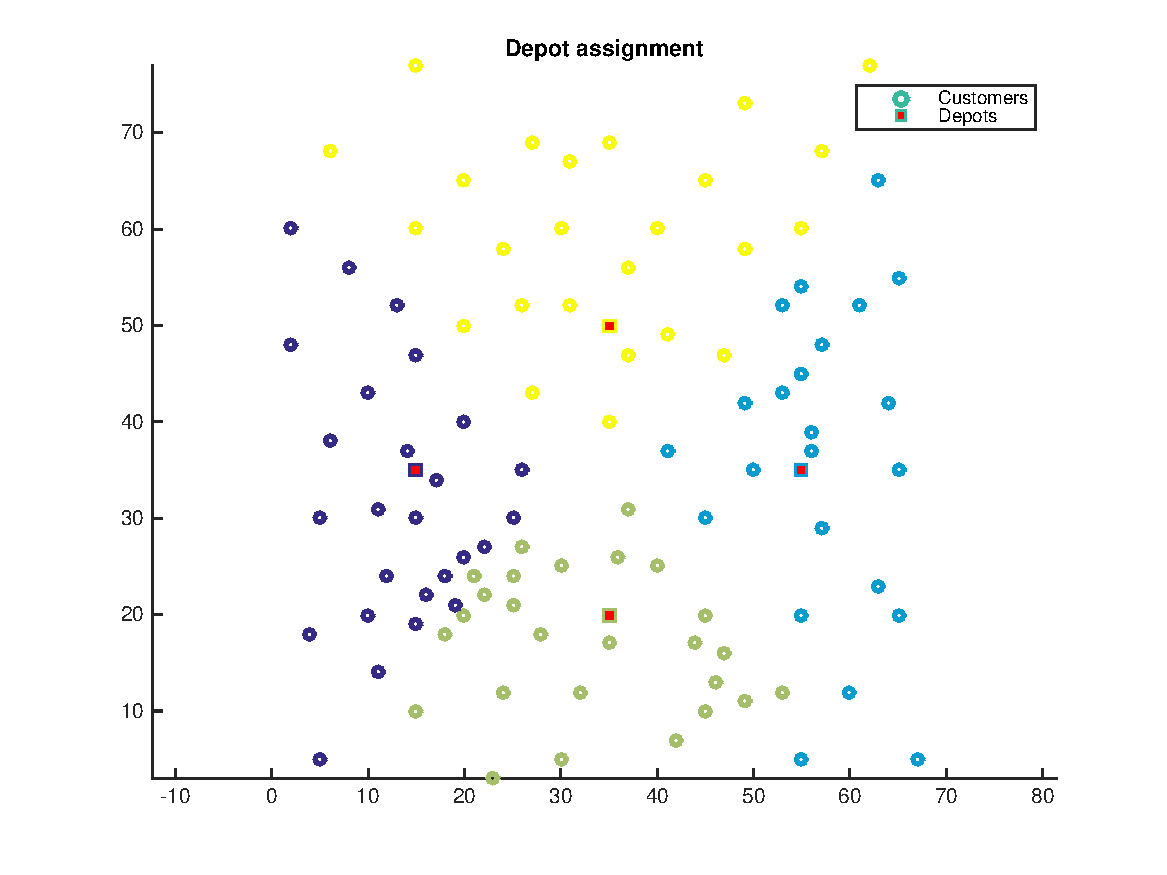
\includegraphics[width=0.32\textwidth]{images/N1depot_assignment}
    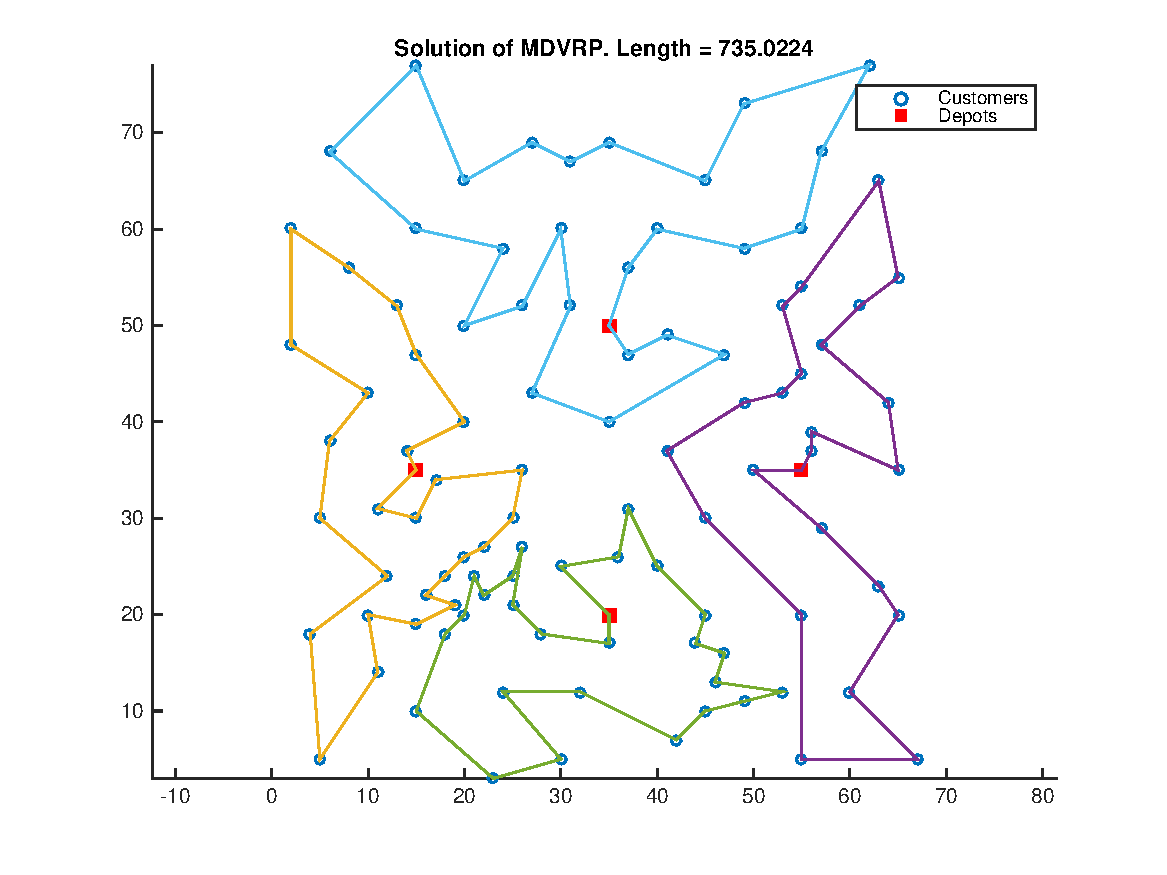
\includegraphics[width=0.32\textwidth]{images/N1solution}
    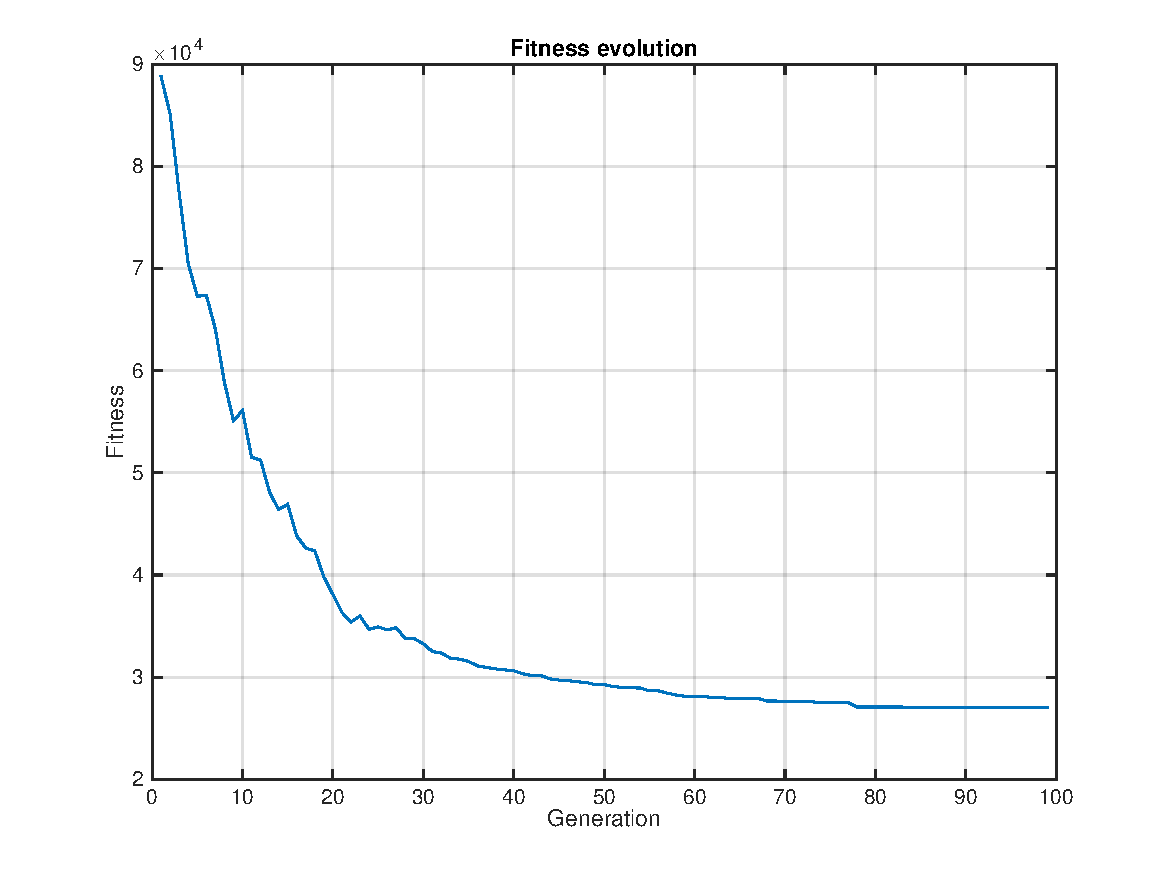
\includegraphics[width=0.32\textwidth]{images/N1fitness}
    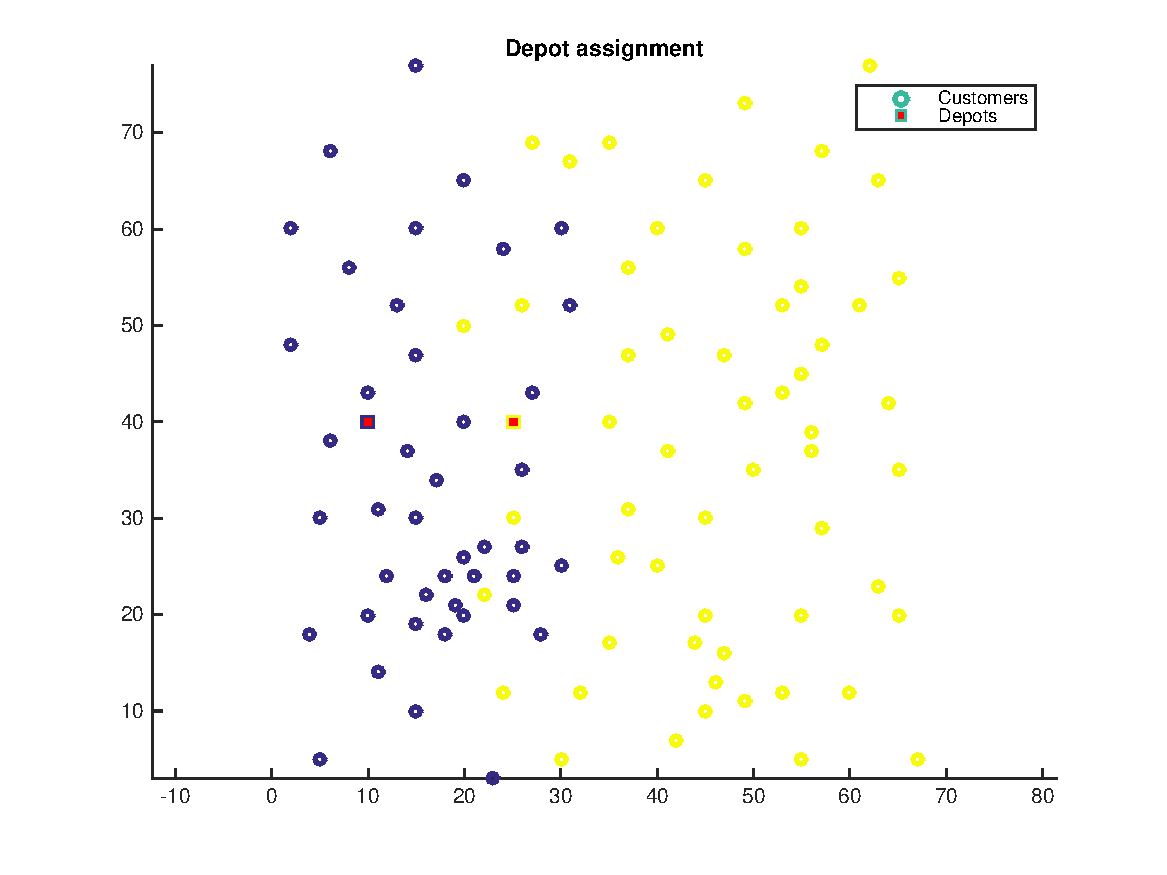
\includegraphics[width=0.32\textwidth]{images/N1depot_assignment_p07altered}
    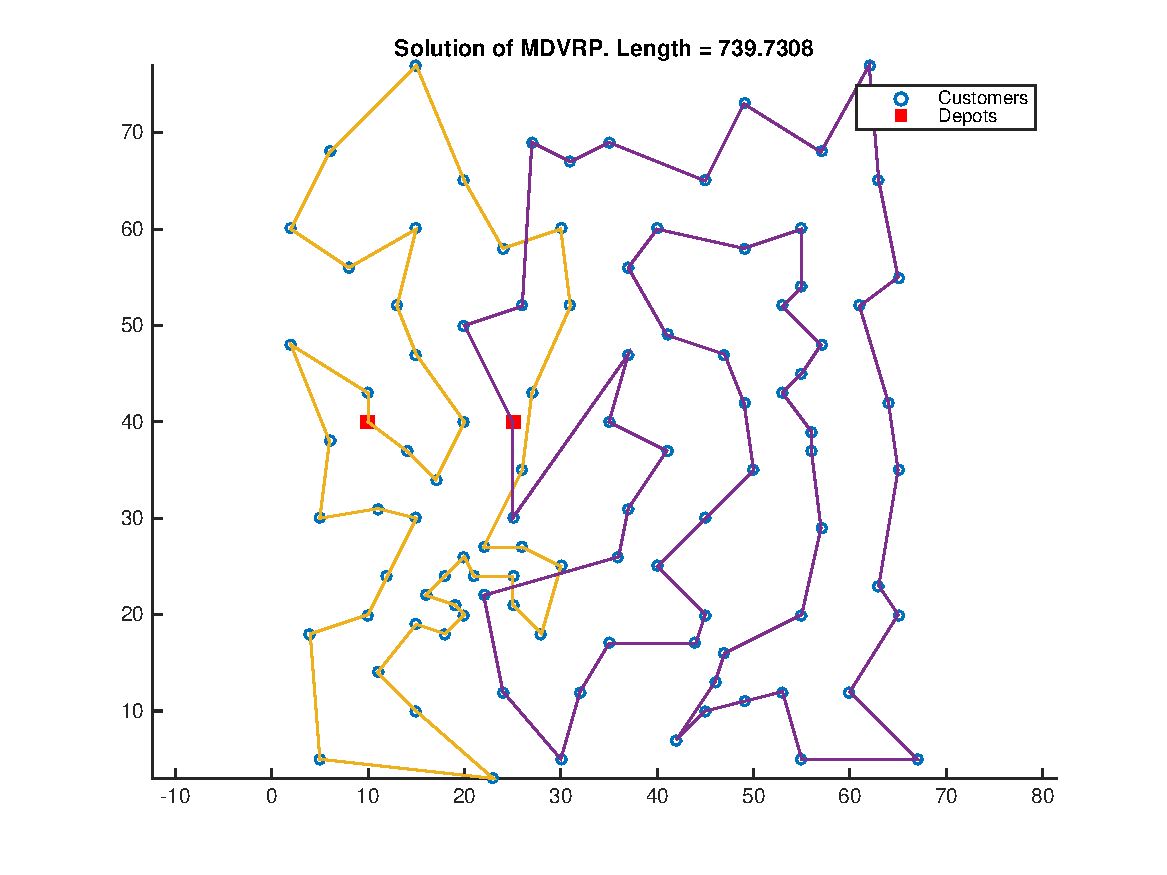
\includegraphics[width=0.32\textwidth]{images/N1solution_p07altered}
    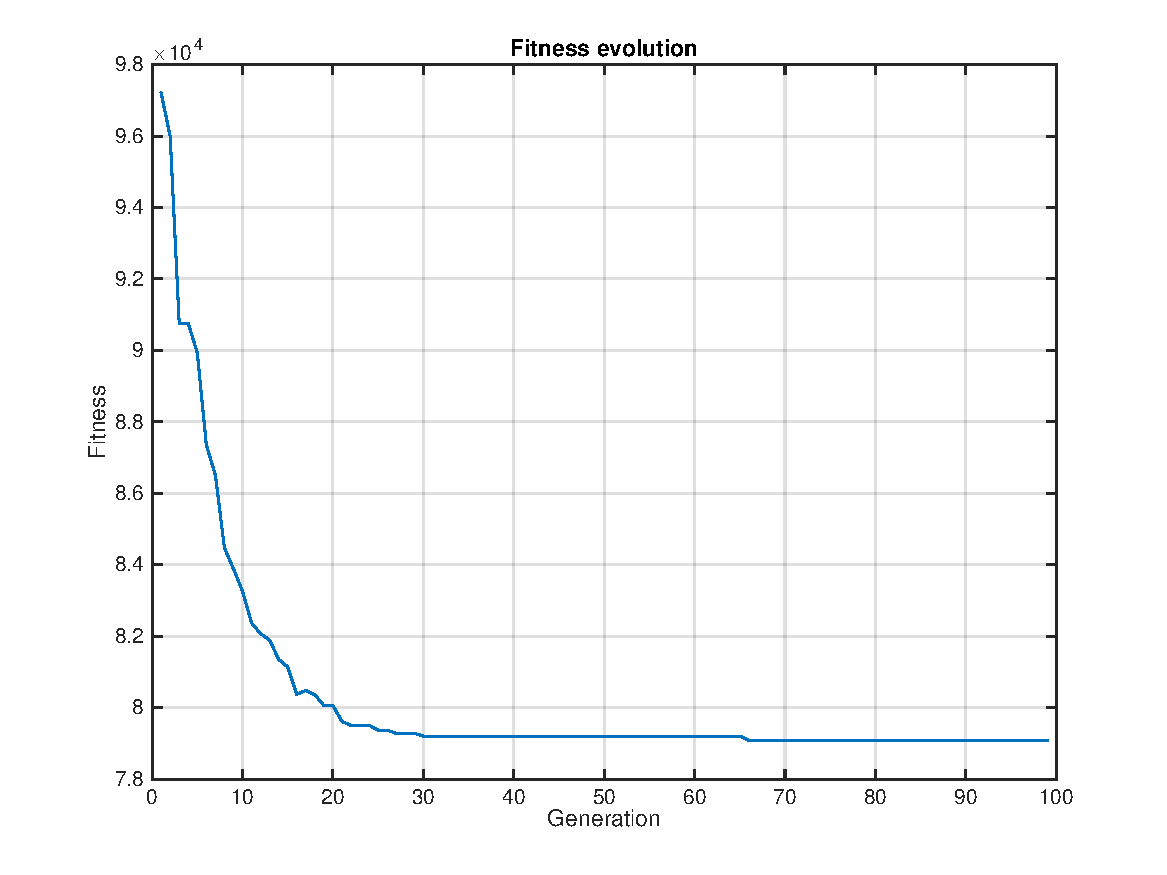
\includegraphics[width=0.32\textwidth]{images/N1fitness_p07altered}
    \caption{Sample results of genetic clustering with Distance to The Depot fitness (\texttt{p07} - top, \texttt{p07altered} - bottom)}
    \label{n1res}
  \end{center}
\end{figure*}

MDVRP results with our competing genetic clustering method are shown in Figure \ref{n3res}. It is obvious that the results of MDVRP are in this case inferior to the K-Means clustering results. However, the nice feature of this fitness function is that it actually allows to create clusters which intersect and therefore the routes in the final routing will cross, which cannot happen for K-Means. It gives us a higher planning flexibility by also not fixing the distances to the depots. Clearly, this approach would not be ideal when considering multiple vehicles from each depot, nonetheless that was not our assignment.
\begin{figure*}
  \begin{center}
    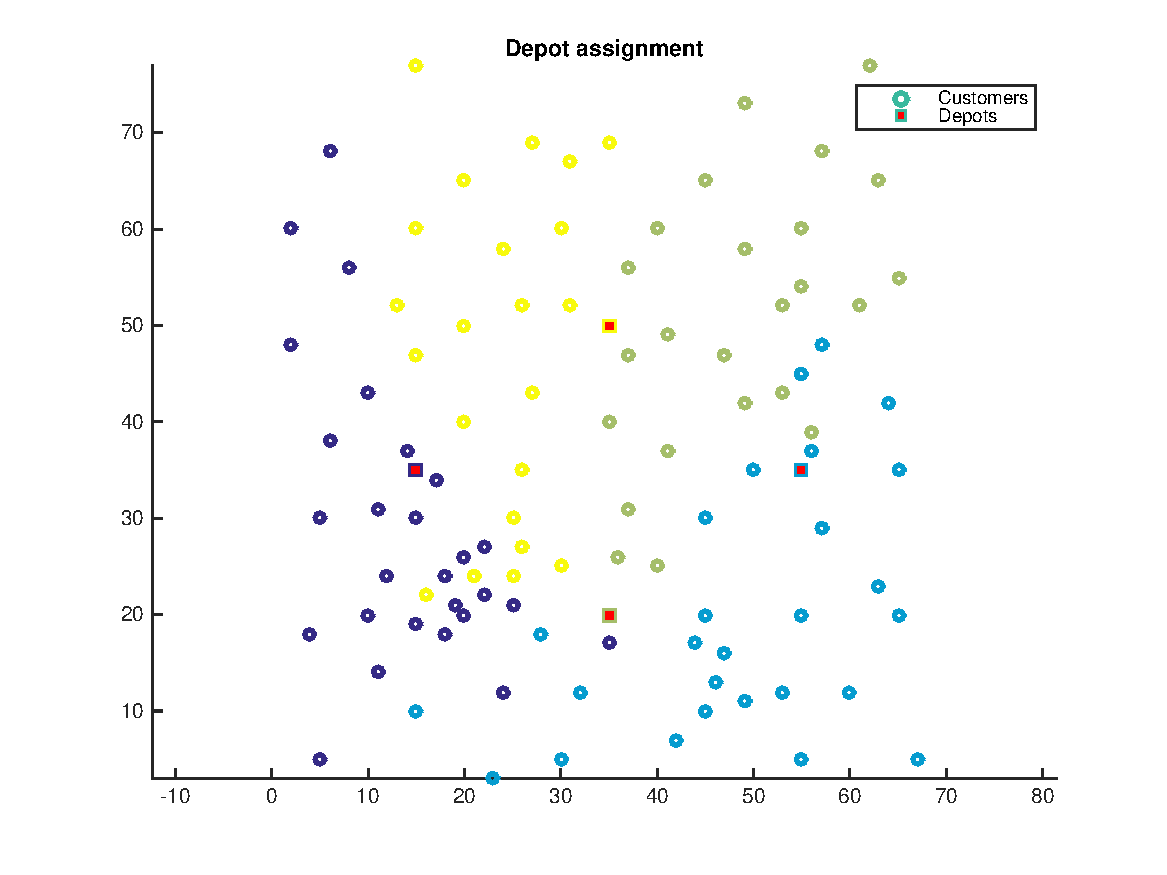
\includegraphics[width=0.32\textwidth]{images/N3depot_assignment2}
    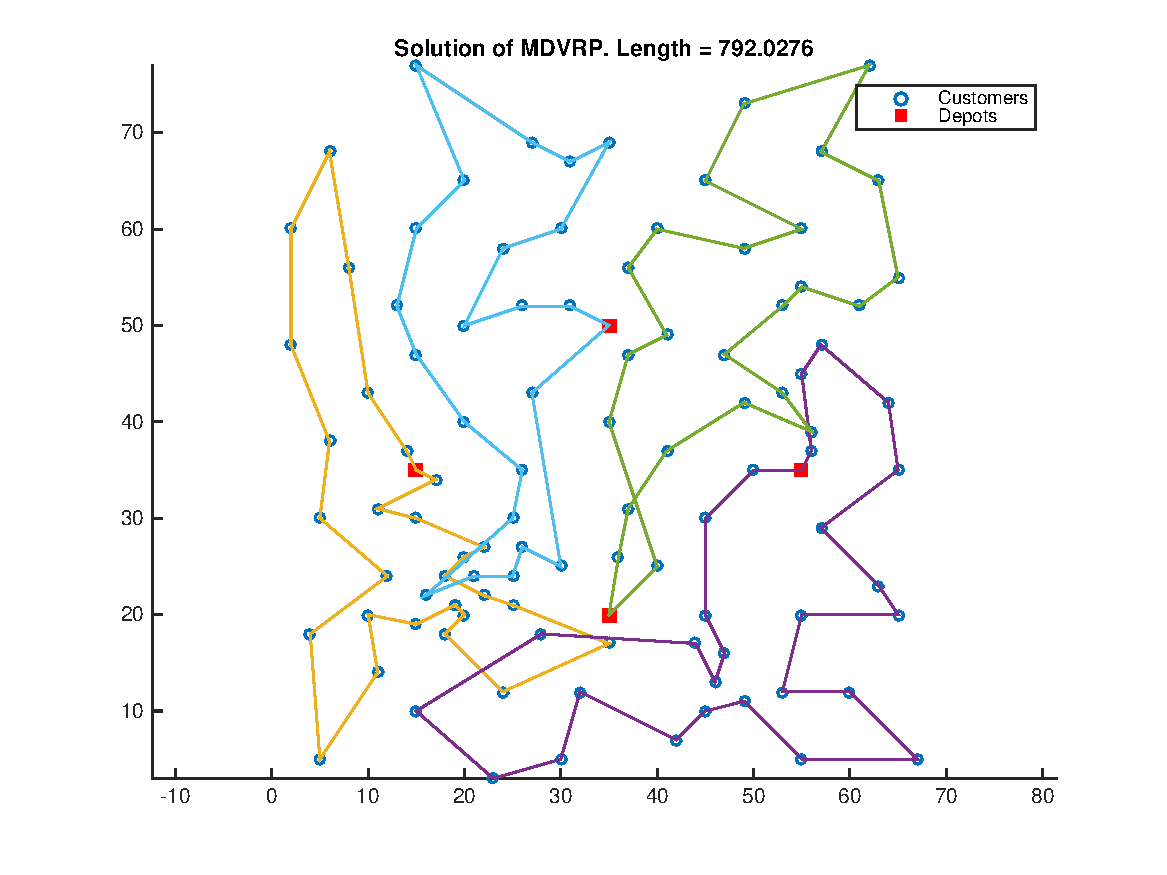
\includegraphics[width=0.32\textwidth]{images/N3solution2}
    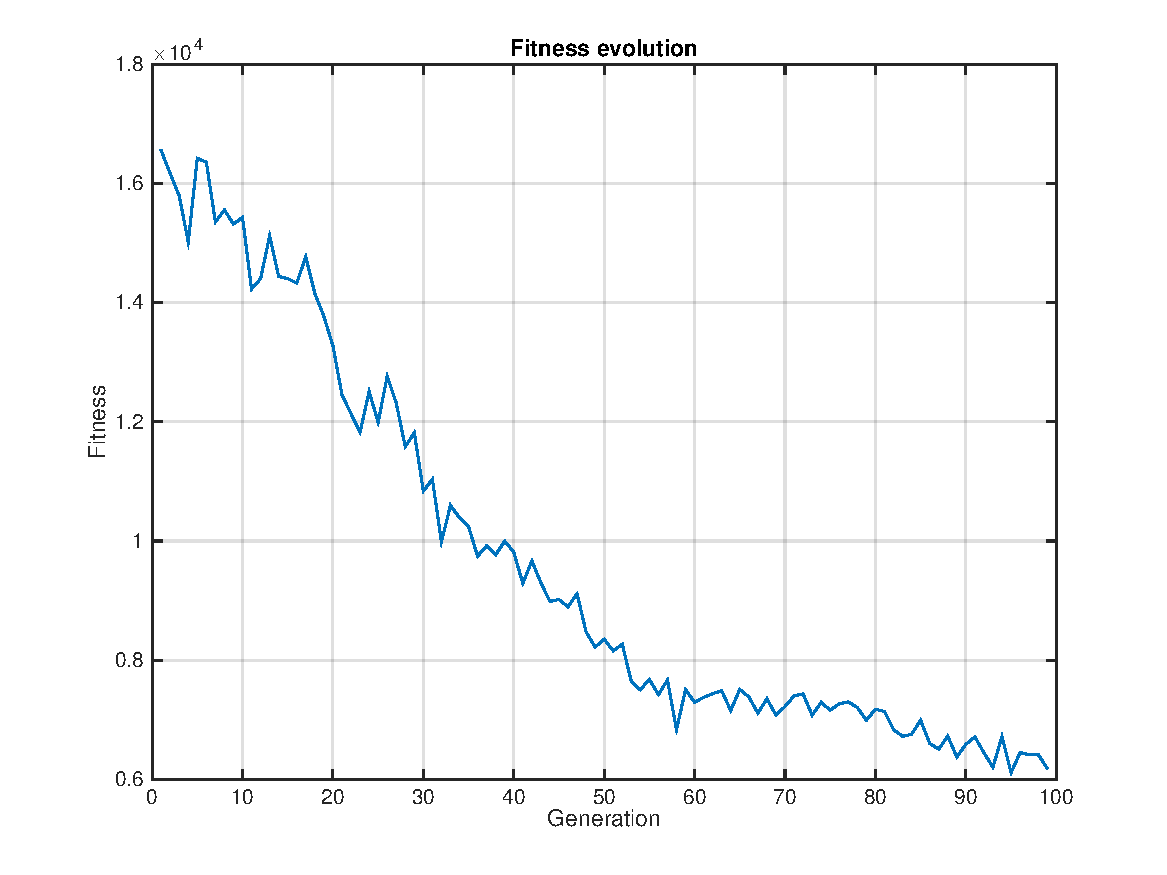
\includegraphics[width=0.32\textwidth]{images/N3fitness2}
    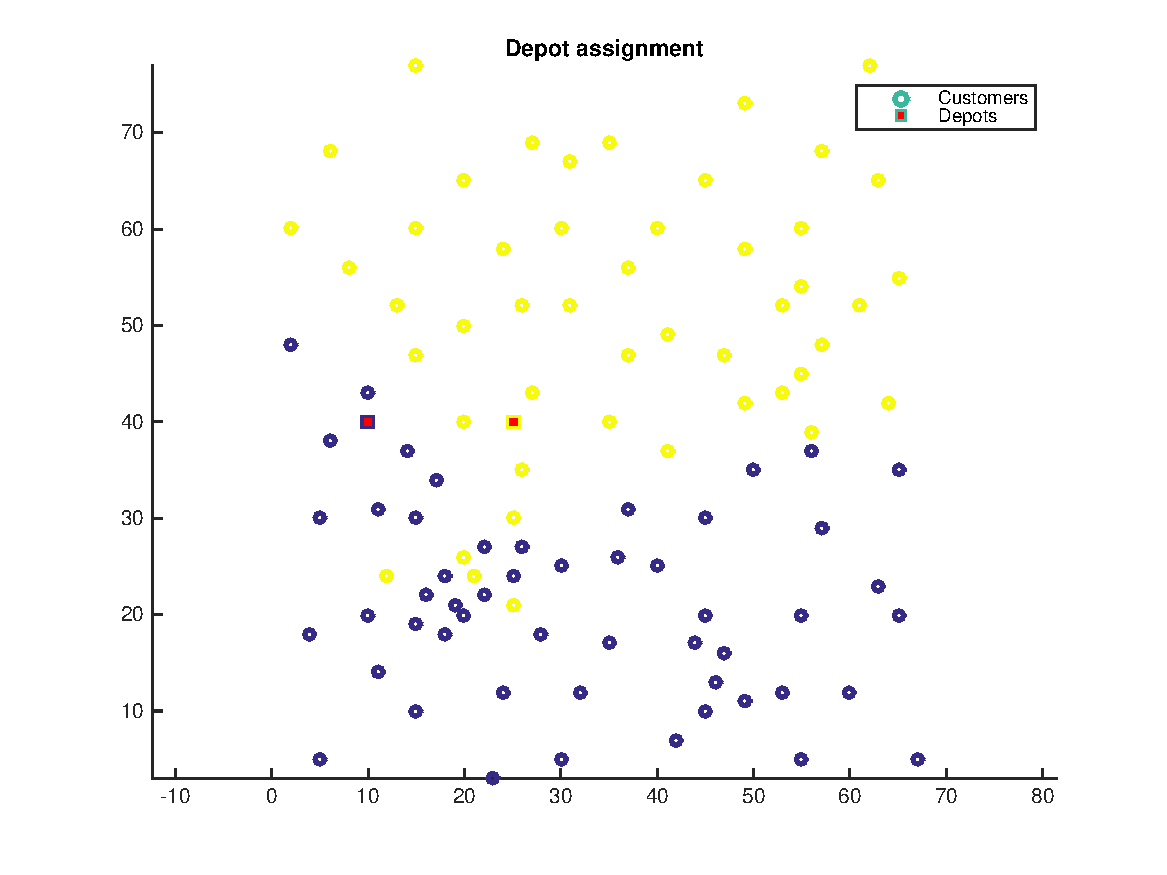
\includegraphics[width=0.32\textwidth]{images/N3depot_assignment_p07altered}
    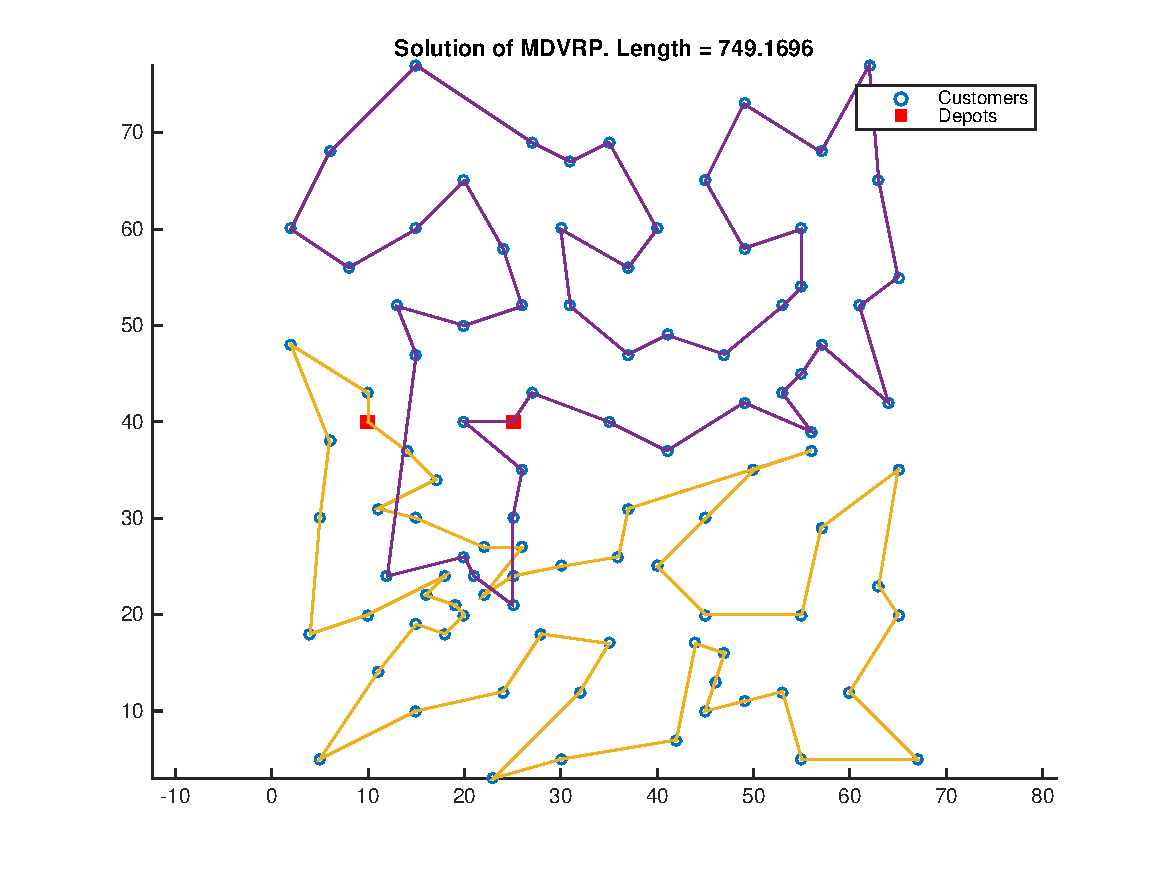
\includegraphics[width=0.32\textwidth]{images/N3solution_p07altered}
    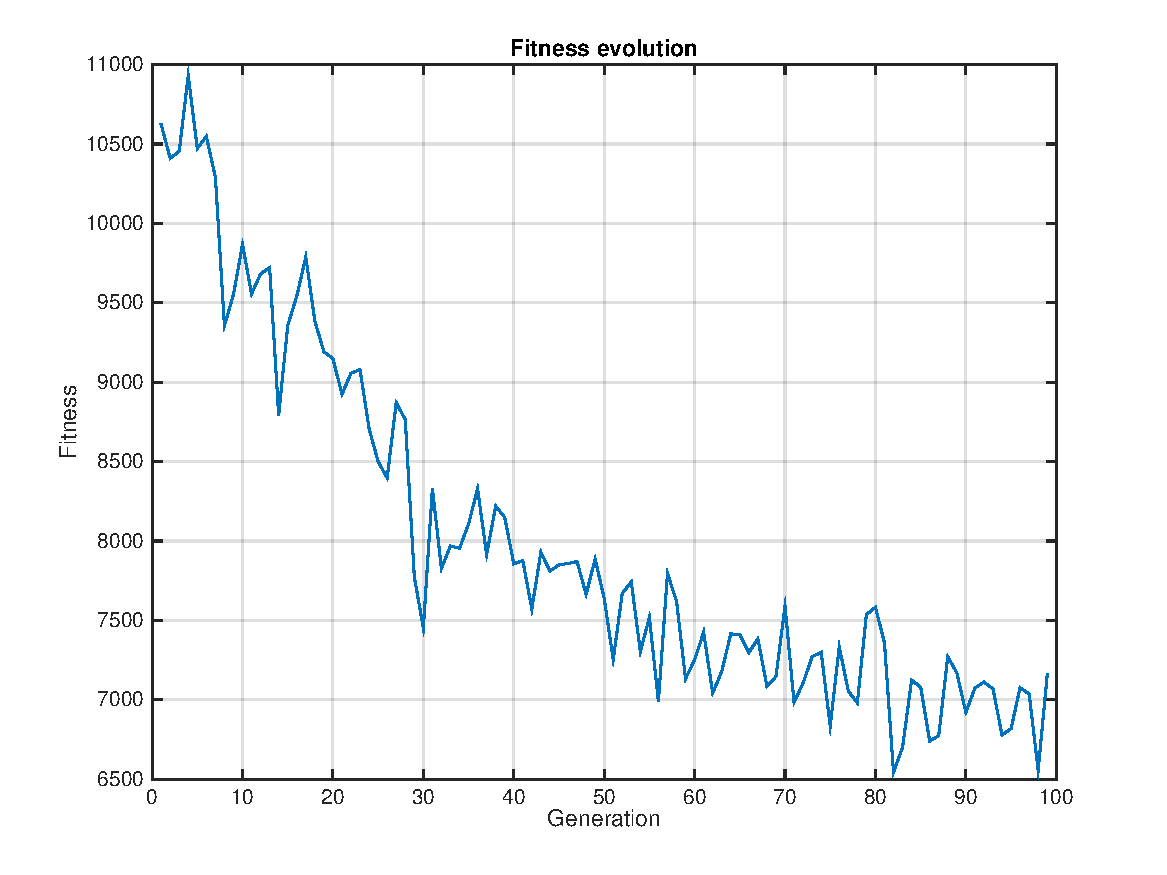
\includegraphics[width=0.32\textwidth]{images/N3fitness_p07altered}
    \caption{Sample results of genetic clustering with Exclusive Pairing fitness (\texttt{p07} - top, \texttt{p07altered} - bottom)}
    \label{n3res}
  \end{center}
\end{figure*}




\section{Discussion}
As is obvious from the results, it was not shown that our suggested fitness function performs better than the original K-Means clustering (Distance to The Depot fitness function). The comparison of the results with used fitness functions is displayed in Table \ref{mcomp}.
\begin{table}[b]
  \begin{center}
    \caption{Comparison of suggested clustering fitness function with K-Means (Distance to The Depot)}
    \begin{tabular}{l | c | c }
     & Distance to The Depot & Exclusive Pairing \\
    \hline
    Instance \texttt{p07}: & 735.02 & 792.03 \\
    \hline
    Instance \texttt{p07altered}: & 739.73 & 741.85 \\
    \hline 
    \end{tabular}
    \label{mcomp}
  \end{center}
\end{table}

However, we can conclude that for a more difficult depot positions our results are very similar to the K-Means ones. The Exclusive Pairing fitness function showed some interesting possibilities for multi depot vehicle routing that the previous methods do not allow. For example creating clusters, which allow for intersecting roads. We believe that a further investigation of this method could lead in some instances to better results than the classical and for MDVRP so widely used K-Means clustering.



\section{Conclusion}
In this semestral work we explored the impact of different clustering methods on the solution of MDVRP. We explained that all regular clustering methods yield the same clusters since the positions of the depots (cluster centers) are given. Hence we proposed a new clustering method that uses genetic algorithms and has a better insight in what actually is the purpose of the clustering.

From the presented results we can conclude that our proposed genetic clustering was not superior to the K-Means strategy. Even though, we showed an interesting new method, which allows for a higher cluster variability then K-Means. It is important because our goal is not to create compact clusters, but clusters suitable for routing.




\nocite{*} % invokes all articles from the bib file
\bibliographystyle{IEEEtran}
\bibliography{references}

\end{document}
